\documentclass[letterpaper,11pt,dvipsnames]{article}	
\usepackage[mathscr]{eucal}
\usepackage[spanish]{babel}
%\usepackage[latin1]{inputenc} 
\usepackage[utf8]{inputenc} 
\usepackage{amsthm,amsmath,amssymb,amsthm,amscd,amsfonts,amsbsy}
\usepackage{mathrsfs}
\usepackage{color}
\usepackage{xcolor}
\usepackage{textcomp}
\usepackage{fancyhdr,latexsym}
\usepackage{epsfig}
\usepackage{graphicx}
\usepackage{subcaption}
\usepackage{thumbpdf}
\usepackage{float}
\usepackage{rotating}
\usepackage{setspace}
\usepackage{multicol}
\usepackage{listings}
\usepackage{hyperref}
\usepackage{multido}
\usepackage{multirow}
\usepackage{tabularx,booktabs,caption}
\usepackage{pgfplots}
\usepackage{curves}
\usepackage[pass]{geometry}
\usepackage[most]{tcolorbox} % Para generar textos con caja de color
\usepackage{calrsfs} %fuente caligrafica estilizada
\pagestyle{plain}
\lstset{
  language=R,
  basicstyle=\ttfamily\small,
  commentstyle=\itshape\color{green!60!black},
  keywordstyle=\bfseries\color{blue},
  numbers=left,
  numberstyle=\tiny\color{gray},
  frame=single,
  breaklines=true,
  captionpos=b,
  showstringspaces=false,
  escapeinside={(*@}{@*)}
}
\newtheorem{theorem}{Teorema}
\newtheorem{exercise}{Ejercicio}
\newtheorem{example}{Ejemplo}
\newtheorem{definition}{Definición}
%se pueden mofificar/agregar mas comandos segun los ambientes necesarios

\addtolength{\voffset}{-1.0in} 
\addtolength{\hoffset}{-1.0in}
\addtolength{\textwidth}{2.0in} 
\addtolength{\textheight}{1.751in}

\title{Práctica 2: Manos de Poker}
\author{Maximiliano Barajas Sánchez}
\begin{document}
\maketitle

%los logotipos oficiales de la institucion se pueden descargar desde
% https://www.comunicacionsocial.uam.mx/identidaduam/html/descargas.html
\begin{picture}(1,1)(0,0)
\put(0,90){
\includegraphics[scale=0.485,keepaspectratio=true]{variacion5Cua.png}}
\end{picture}
\section{Introducción}
A lo largo de esta práctica se analizarán las diversas manos del juego de Poker así como el problema de conteo detrás del mismo juego como un pequeño análisis sobre una cantidad considerable de partidas del juego realizadas en el laboratorio.
\section{Metodología}
Inicialmente se realizará el problema de conteo con el cual podemos calcular las probabilidades de cada mano, a continuación realizaremos una cantidad de partidas considerables registrando las manos obtenidas en una tabla de frecuencias que finalmente se analizará con ayuda de R.
\section{Marco teórico}
Comenzamos planteando el problema de conteo para cada categoría de mano, nosotros consideramos escalera real, escalera de color, poker, full house, color, escalera, tercia, doble par, par y carta alta. Iniciamos calculando todas las posibles manos, las cuales resultan en 
\({{52}\choose{5}}\), esta es la cardinalidad de nuestro espacio muestral que representa el total de todas las posibles manos,comenzamos con cada mano.
\subsection{Escalera Real}
En este caso tenemos 4 formas en 1 de elegir el palo y por cada una de ellas tenemos 5 formas en 5 de elegir las 5 cartas restantes lo que resulta en \({{4}\choose{1}}{{5}\choose{5}}=4\) formas de conseguir una escalera real, esto resulta en una probabilidad de \(1.539077 \times 10^{-6}\) .
\subsection{Escalera de color}
En este caso tenemos nuevamente 4 en 1 formas de escoger el palo y por cada una de ellas tenemos 9 formas de elegir el primer número de la escalera para excluir la escalera real lo que resulta en \({{4}\choose{1}}9=36\) formas posibles, que se traducen en una probabilidad de \(1.3851\times 10^{-5}\) .
\subsection{Poker}
Para este caso tenemos 13 en 1 formas de elegir el primer número y por cada una de esas formas tenemos 4 en 4 formas de elegir el palo y para la carta restante tenemos 12 en 1 formas de elegir el número y 4 en 1 formas de elegir el palo lo que resulta en \({{13}\choose{1}}{{4}\choose{4}}{{12}\choose{1}}{{4}\choose{1}}=624\) con una probabilidad de aproximadamente  \(2.4009 \times 10^{-4}\)
\subsection{Full House}
En este caso tenemos 13 en 1 formas de elegir el número inicial, 4 en 3 formas de elegir el palo de las primeras tres cartas, 12 en 1 formas de elegir el número de la pareja y 4 en 2 formas de elegir el palo de dicha pareja resultando en \({{13}\choose{1}}{{4}\choose{3}}{{12}\choose{1}}{{4}\choose{2}}=3744\) formas con una probabilidad de \(1.4405 \times 10^{-3}\)
\subsection{Color}
Inicialmente elegimos los posibles números los cuales son 13 en 5 formas y el palo que debe ser el mismo que resulta en 4 en 1 formas y a estas formas tenemos que restarles la flor imperial y la escalera color que entranen el conteo inicial, esto resulta en después de simplificar en \({{13}\choose{5}}{{4}\choose{1}}-10{{4}\choose{1}}=5108\) con una probabilidad de \(1.9654 \times 10^{-3}\)
\subsection{Escalera}
En este caso tenemos 10 en 1 formas de elegir el primer número de la escalera y los palos de las cartas que conforman la escalera son las de 4 en 1 elevadas a la potencia 5, debemos restar la escalera real y la escalera color  como en el caso anterior, esto resulta en un total de \({{10}\choose{1}}{{4}\choose{1}}^{5}-10{{4}\choose{1}}=10200\)con una probabilidad de \(3.9246 \times 10^{-3}\)
\subsection{Tercia}
En este caso tenemos 13 en 1 maneras de elegir el número de la tercia y 4 en 3 formas de elegir el palo de cada carta, tenemos 12 en 2 formas de elegir las 2 cartas restrantes y 4 en 1 formas de elegir el palo de cada una por lo que lo elevamos al cuadrado, esto resulta en \({{13}\choose{1}}{{4}\choose{3}}{{12}\choose{2}}{{4}\choose{3}}^{2}=54912\) con una probabilidad de 0.0211284 aproximadamente.
\subsection{Doble par}
Aqui tenemos 13 en 2 formas de elegir los números, 4 en 2 formas de elegir los palos, como son dos pares lo elevamos al cuadrado y para la carta restante hay 11 en 1 formas de elegir el número y 4 en 1 formas de elegir el palo, esto resulta en \({{13}\choose{2}}{{4}\choose{2}}^{2}{{11}\choose{1}}{{4}\choose{1}}=123552\) formas con una probabilidad de 0.047539
\subsection{Par}
Aquí tenemos 13 en un formas de elegir el número, 4 en dos formas de elegir el palo del par y 12 en 3 formas de elegir los 3 números restantes y 4 en 1 formas de elegir los palos de cada una de esas tres cartas por lo que obtenemos \({{13}\choose{1}}{{4}\choose{2}}{{12}\choose{3}}{{4}\choose{3}}^{3}=1098240\) formas con una probabilidad de 0.42256  aproximadamente.
\subsection{Carta alta}
En este caso decidí usar la bibliografía dado que es un cálculo extremadamente largo, la bibliografía indica que son 1302540 con una probabilidad de 0.501177
Ya que hemos respondido las preguntas iniciales con el apartado anterior del marco teórico en cuanto a la probabilidad de cada una de las manos obtenidas y su probabilidad procedemos a responder la última pregunta que es cómo calculamos la probabilidad de la siguiente mano a mi parecer esto puede realizarse con el teorema de Bayes de proibabilidad condicional.
\section{Discusión}
En cuanto a nuestros resultados generamos la siguiente tabla de resultados, fue a través de una hoja de cálculo que mas tarde exportamos a un Script de R, aqui se encuentra la tabla a continuación:
\begin{figure}[H]
    \centering
    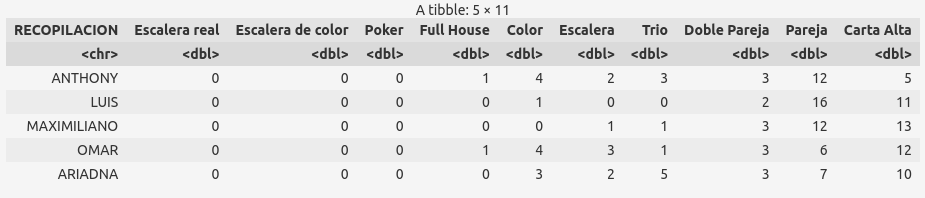
\includegraphics[scale=0.485]{tabla.png}
    \caption{Tabla de datos}
    \label{fig:hipocicloide}
\end{figure}
A continuación mostramos las gráficas que yo personalmente decidí realizar sobre estos resultados:
\begin{figure}[H]
    \centering
    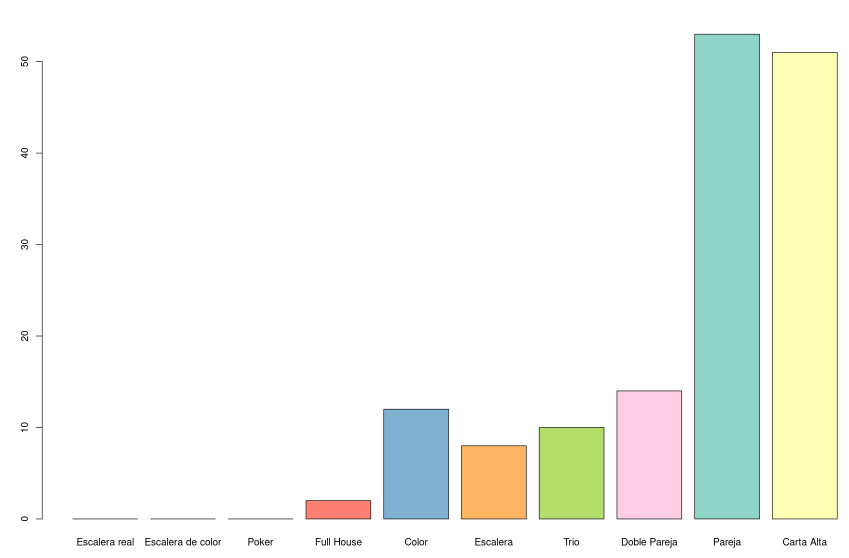
\includegraphics[scale=0.485]{barras.png}
    \caption{Tabla de datos}
    \label{fig:hipocicloide}
\end{figure}
Notamos que la frecuencia de cada tipo de mano después de realizar 30 partidas es bastante similar a la frecuencia relativa esperada que calculamos en el marco teórico siendo la pareja y la carta alta las de mayor recurrencia, también decidí hacer una gráfica de pastel:

\begin{figure}[H]
    \centering
    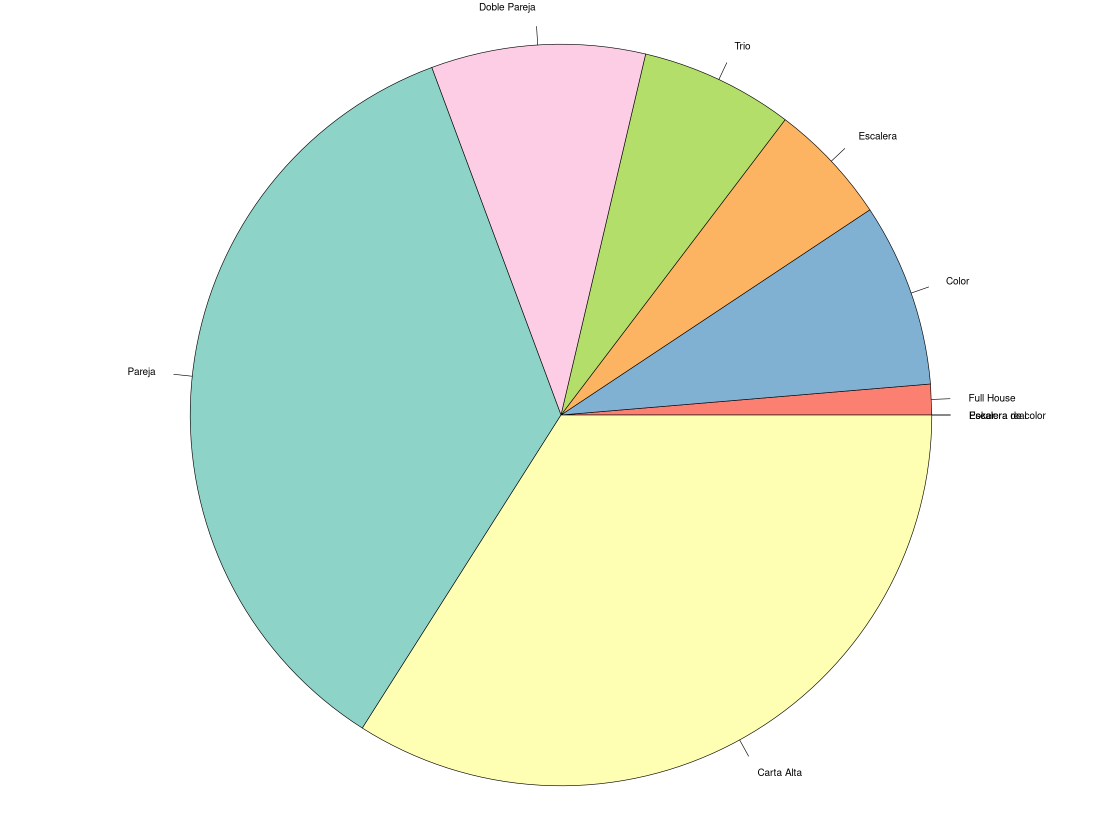
\includegraphics[scale=0.485]{pie.png}
    \caption{Tabla de datos}
    \label{fig:hipocicloide}
\end{figure}
Podemos observar en la gráfica de pastel de forma mucho mas clara la frecuencia relativa de cada mano respecto a las demás, nuevamente asemejándose a la frecuencia establecida en el apartado teórico de la práctica, finalmente a consejo de la bibliografía decidí realizar una gráfica de araña o bien una "scatterpolar" plot la cual resultó en el siguiente material gráfico, se realizó con ayuda de plotly para R, el código esta adjunto a la entrega en un jupyter Notebook.
\begin{figure}[H]
    \centering
    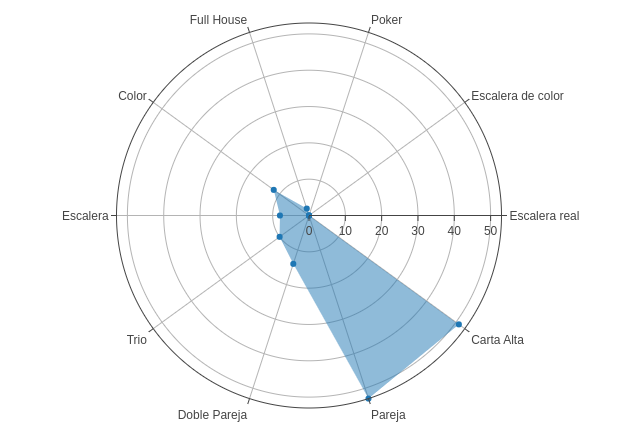
\includegraphics[scale=0.485]{spider.png}
    \caption{Tabla de datos}
    \label{fig:hipocicloide}
\end{figure}
Nuevamente podemos observar la desproporción esperada de la frecuencia de cada tipo de mano, en lo personal considero que este tipo de gráfica es bastante mas llamativa visualmente y de igual manera mucho mas sencilla de interpretar en cuanto a frecuencias relativas respecta.
\section{Conclusiones} 
Finalmente puedo concluir que la realización como manipulación adecuada de los datos experimentales de cualquier tipo es de vital importancia al igual que el cuidado en la realización de cualquier tipo de experimento, durante la práctca en el laboratorio se presentaron errores como reusar cartas de manos pasadas en la misma partida lo que resulto en tener que repetir partidas desde 0, por otra parte en cuanto al como podemos aplicar esto podemos interpretar el evento de que aparezcan ciertas manos en una partida de un valor considerable en particular yo pienso que a partir de las escaleras de tal suerte que posamos tratar de asumir que podriamos esperar en el turno siguiente o de las manos de nuestros contrincantes.
\section*{Referencias Bibliográficas}
\begin{enumerate}
    \item Castillo, P., & de Lourdes, M. (1999). Probabilities and simulations in poker.
    \item Korb, K. B., Nicholson, A., & Jitnah, N. (2013). Bayesian poker. arXiv preprint arXiv:1301.6711.
    \item George F. Simmons (1992). Calculus Gems. Chapter B.21: The Cycloid.
    \item Ambekar, G., Chikane, T., Sheth, S., Sable, A., & Ghag, K. (2015, September). Anticipation of winning probability in poker using data mining. In 2015 International Conference on Computer, Communication and Control (IC4) (pp. 1-6). IEEE.
    \item Rubin, J., & Watson, I. (2011). Computer poker: A review. Artificial intelligence, 175(5-6), 958-987.
    
\end{enumerate}
\end{document}
%=================
\end{document}
%===========================================================================================
_______________________________FIN DEL DOCUMENTO___________________________________________
%===========================================================================================
